\subsection{Fourth problem}


\begin{figure}[H]
    \centering    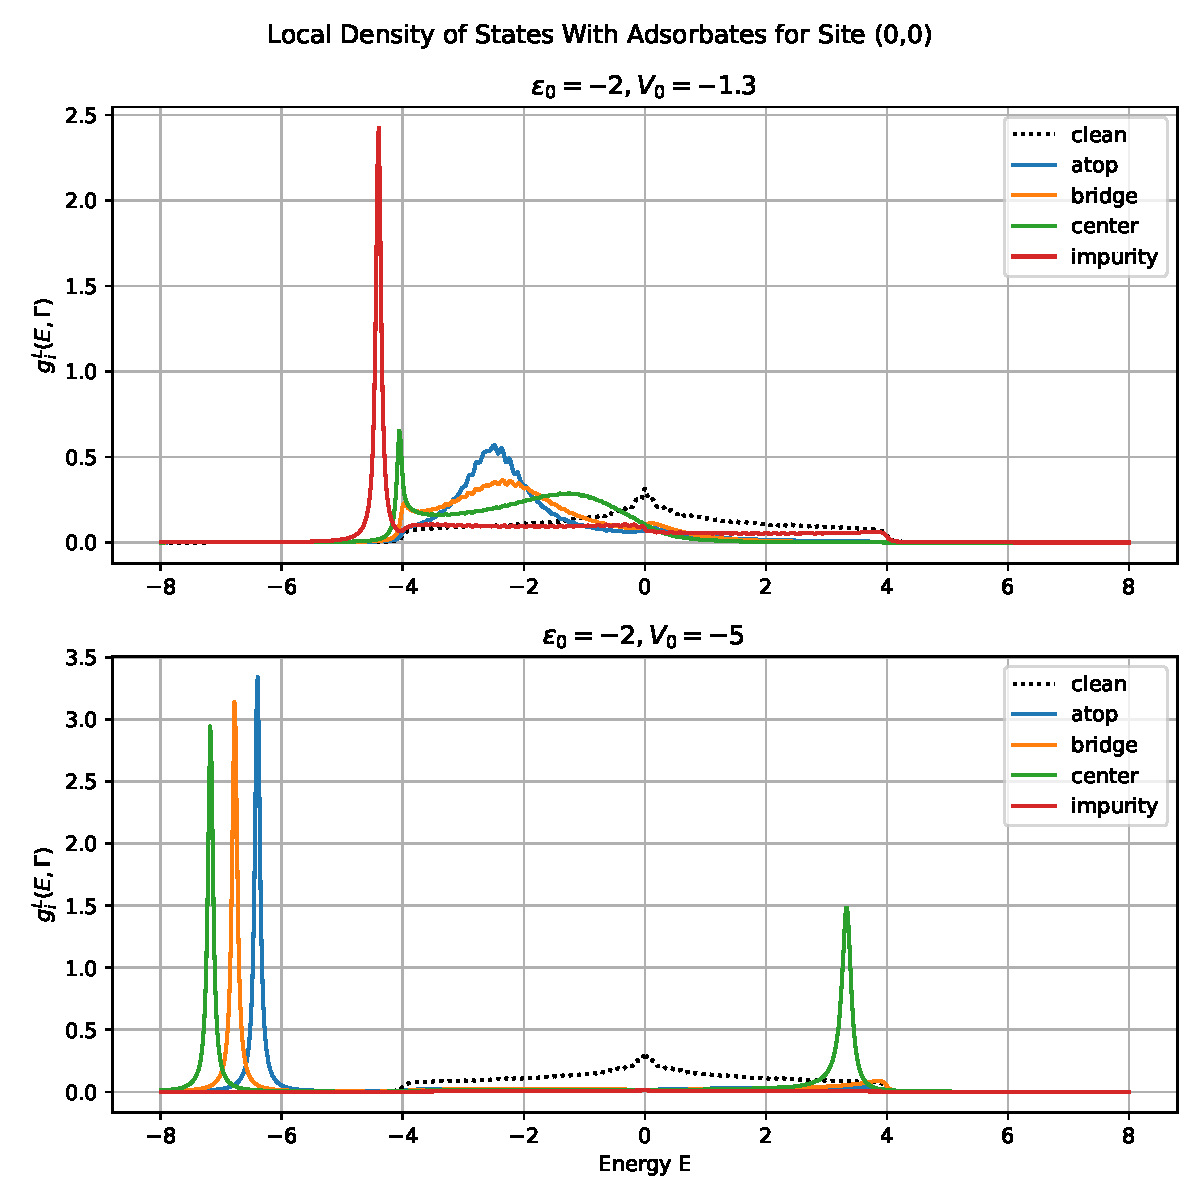
\includegraphics[width=\textwidth]{Figures/task4-11.pdf}
    \caption{Zoomed in plot of the LDOS at site (0,0) for a 2D square lattice with and without adsorbates for two sets of parameters, $\epsilon_0=-2,\:V_0=-1.3$ and $\epsilon_0=-2,\:V_0=-5$}
    \label{fig:task4}
\end{figure}


\begin{figure}[H]
    \centering    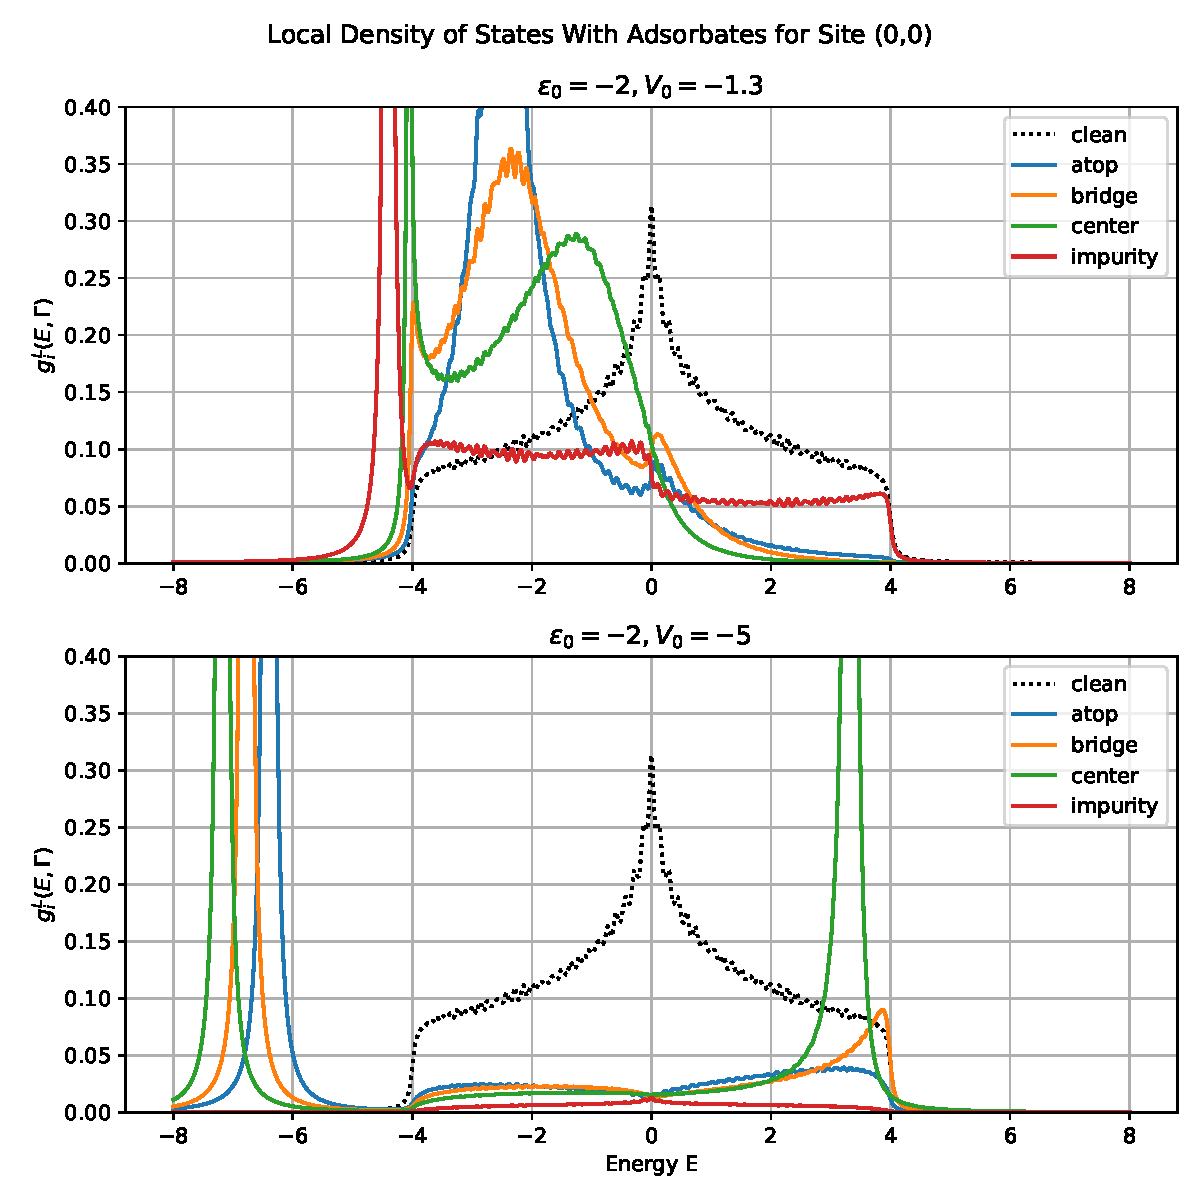
\includegraphics[width=\textwidth]{Figures/task4-11(1).pdf}
    \caption{LDOS at site (0,0) for a 2D square lattice with and without adsorbates for two sets of parameters, $\epsilon_0=-2,\:V_0=-1.3$ and $\epsilon_0=-2,\:V_0=-5$}
    \label{fig:task4(1)}
\end{figure}

\begin{figure}[H]
    \centering    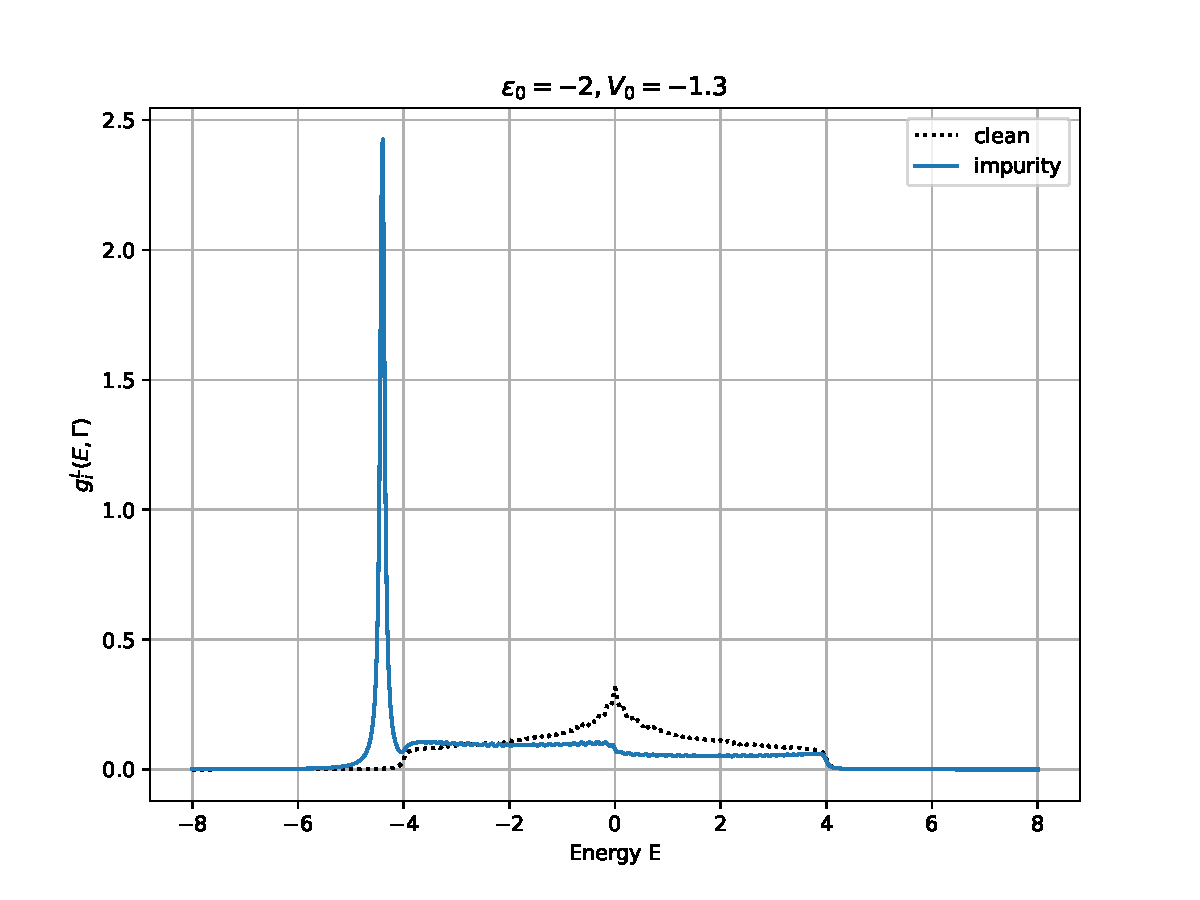
\includegraphics[width=\textwidth]{Figures/task4-imp.pdf}
    \caption{LDOS at the (0,0) site for a clean surface and for the impurity case, where the surface atom is replaced by an adsorbate with $\epsilon_0=-2,\:V_0=-1.3$.}
    \label{fig:task4imp}
\end{figure}

\textbf{A4}
\\
1) When $V_0$ is weak the adsorbate has a smaller effect on the surface LDOS and its own LDOS is more localized near its own energy level. However, when $V_0$ is stronger the adorbate interacts more strongly with the surface and significantly modifies the LDOS of both the surface and the adsorbate.  

2) Yes the LDOS is adsorption-site sensitive for both parameters since an adsorption is present. However the sensitivity decreases as the coupling strength increases due to stronger hybridization effects, so for the $\epsilon_0=-2,\:V_0=-5$ parameter is not as absorption-site sensitive the strong coupling dominates over site-dependent variations.

3) In figure \ref{fig:task4imp}, the LDOS of the impurity case shifted towards lower energies compared to that of the clean surface. Additionally in the impurity case, the hopping to nearest neighbors, $V_0=-1.3$, has changed compared to the bulk one thus resulting in the sharper and more pronounced peak compared to the symmetric one for the clean case.

4) For question 2, the adsorption-site sensitivity would remain qualitatively similar. However the LDOS at distant sites should become independent of the adsorbates presence since its impact would decay spatially. Regarding question 3, the difference between the impurity site and the surrounding clean surface would be maintained locally. In other words, going away from the impurity the LDOS will recover the clean-surface profile while the impurity’s effect remains a local perturbation.